\documentclass{beamer}

\pdfmapfile{+sansmathaccent.map}


\mode<presentation>
{
	\usetheme{Warsaw} % or try Darmstadt, Madrid, Warsaw, Rochester, CambridgeUS, ...
	\usecolortheme{seahorse} % or try seahorse, beaver, crane, wolverine, ...
	\usefonttheme{serif}  % or try serif, structurebold, ...
	\setbeamertemplate{navigation symbols}{}
	\setbeamertemplate{caption}[numbered]
} 


%%%%%%%%%%%%%%%%%%%%%%%%%%%%
% itemize settings


%%%%%%%%%%%%%%%%%%%%%%%%%%%%
% itemize settings

\definecolor{myhotpink}{RGB}{255, 80, 200}
\definecolor{mywarmpink}{RGB}{255, 60, 160}
\definecolor{mylightpink}{RGB}{255, 80, 200}
\definecolor{mypink}{RGB}{255, 30, 80}
\definecolor{mydarkpink}{RGB}{155, 25, 60}

\definecolor{mypaleblue}{RGB}{240, 240, 255}
\definecolor{mylightblue}{RGB}{120, 150, 255}
\definecolor{myblue}{RGB}{90, 90, 255}
\definecolor{mygblue}{RGB}{70, 110, 240}
\definecolor{mydarkblue}{RGB}{0, 0, 180}
\definecolor{myblackblue}{RGB}{40, 40, 120}

\definecolor{myblackturquoise}{RGB}{5, 53, 60}
\definecolor{mydarkdarkturquoise}{RGB}{8, 93, 110}
\definecolor{mydarkturquoise}{RGB}{28, 143, 150}
\definecolor{mypaleturquoise}{RGB}{230, 255, 255}
\definecolor{myturquoise}{RGB}{48, 213, 200}

\definecolor{mygreen}{RGB}{0, 200, 0}
\definecolor{mydarkgreen}{RGB}{0, 120, 0}
\definecolor{mygreen2}{RGB}{245, 255, 230}

\definecolor{mygrey}{RGB}{120, 120, 120}
\definecolor{mypalegrey}{RGB}{160, 160, 160}
\definecolor{mydarkgrey}{RGB}{80, 80, 160}

\definecolor{mydarkred}{RGB}{160, 30, 30}
\definecolor{mylightred}{RGB}{255, 150, 150}
\definecolor{myred}{RGB}{200, 110, 110}
\definecolor{myblackred}{RGB}{120, 40, 40}

\definecolor{mygreen}{RGB}{0, 200, 0}
\definecolor{mygreen2}{RGB}{205, 255, 200}

\definecolor{mydarkcolor}{RGB}{60, 25, 155}
\definecolor{mylightcolor}{RGB}{130, 180, 250}

\setbeamertemplate{itemize items}[default]

\setbeamertemplate{itemize item}{\color{myblackturquoise}$\blacksquare$}
\setbeamertemplate{itemize subitem}{\color{mydarkdarkturquoise}$\blacktriangleright$}
\setbeamertemplate{itemize subsubitem}{\color{mygray}$\blacksquare$}

\setbeamercolor{palette quaternary}{fg=white,bg=myblackturquoise}
\setbeamercolor{titlelike}{parent=palette quaternary}

\setbeamercolor{palette quaternary2}{fg=black,bg=mypaleblue}
\setbeamercolor{frametitle}{parent=palette quaternary2}

\setbeamerfont{frametitle}{size=\Large,series=\scshape}
\setbeamerfont{framesubtitle}{size=\normalsize,series=\upshape}





%%%%%%%%%%%%%%%%%%%%%%%%%%%%
% block settings

\setbeamercolor{block title}{bg=red!30,fg=black}

\setbeamercolor*{block title example}{bg=mygreen!40!white,fg=black}

\setbeamercolor*{block body example}{fg= black, bg= mygreen2}


%%%%%%%%%%%%%%%%%%%%%%%%%%%%
% URL settings
\hypersetup{
	colorlinks=true,
	linkcolor=blue,
	filecolor=blue,      
	urlcolor=blue,
}

%%%%%%%%%%%%%%%%%%%%%%%%%%

\renewcommand{\familydefault}{\rmdefault}

\usepackage{amsmath}
\usepackage{mathtools}

\usepackage{subcaption}

\usepackage{qrcode}

\DeclareMathOperator*{\argmin}{arg\,min}
\newcommand{\bo}[1] {\mathbf{#1}}

\newcommand{\R}{\mathbb{R}} 
\newcommand{\T}{^\top}     



\newcommand{\mydate}{Fall 2023}

\newcommand{\mygit}{\textcolor{blue}{\href{https://github.com/SergeiSa/Control-Theory-Slides-Spring-2023}{github.com/SergeiSa/Control-Theory-Slides-Spring-2023}}}

\newcommand{\myqr}{ \textcolor{black}{\qrcode[height=1.5in]{https://github.com/SergeiSa/Control-Theory-Slides-Spring-2023}}
}

\newcommand{\myqrframe}{
	\begin{frame}
		\centerline{Lecture slides are available via Github, links are on Moodle}
		\bigskip
		\centerline{You can help improve these slides at:}
		\centerline{\mygit}
		\bigskip
		\myqr
	\end{frame}
}


\newcommand{\bref}[2] {\textcolor{blue}{\href{#1}{#2}}}

%%%%%%%%%%%%%%%%%%%%%%%%%%%%
% code settings

\usepackage{listings}
\usepackage{color}
% \definecolor{mygreen}{rgb}{0,0.6,0}
% \definecolor{mygray}{rgb}{0.5,0.5,0.5}
\definecolor{mymauve}{rgb}{0.58,0,0.82}
\lstset{ 
	backgroundcolor=\color{white},   % choose the background color; you must add \usepackage{color} or \usepackage{xcolor}; should come as last argument
	basicstyle=\footnotesize,        % the size of the fonts that are used for the code
	breakatwhitespace=false,         % sets if automatic breaks should only happen at whitespace
	breaklines=true,                 % sets automatic line breaking
	captionpos=b,                    % sets the caption-position to bottom
	commentstyle=\color{mygreen},    % comment style
	deletekeywords={...},            % if you want to delete keywords from the given language
	escapeinside={\%*}{*)},          % if you want to add LaTeX within your code
	extendedchars=true,              % lets you use non-ASCII characters; for 8-bits encodings only, does not work with UTF-8
	firstnumber=0000,                % start line enumeration with line 0000
	frame=single,	                   % adds a frame around the code
	keepspaces=true,                 % keeps spaces in text, useful for keeping indentation of code (possibly needs columns=flexible)
	keywordstyle=\color{blue},       % keyword style
	language=Octave,                 % the language of the code
	morekeywords={*,...},            % if you want to add more keywords to the set
	numbers=left,                    % where to put the line-numbers; possible values are (none, left, right)
	numbersep=5pt,                   % how far the line-numbers are from the code
	numberstyle=\tiny\color{mygray}, % the style that is used for the line-numbers
	rulecolor=\color{black},         % if not set, the frame-color may be changed on line-breaks within not-black text (e.g. comments (green here))
	showspaces=false,                % show spaces everywhere adding particular underscores; it overrides 'showstringspaces'
	showstringspaces=false,          % underline spaces within strings only
	showtabs=false,                  % show tabs within strings adding particular underscores
	stepnumber=2,                    % the step between two line-numbers. If it's 1, each line will be numbered
	stringstyle=\color{mymauve},     % string literal style
	tabsize=2,	                   % sets default tabsize to 2 spaces
	title=\lstname                   % show the filename of files included with \lstinputlisting; also try caption instead of title
}


%%%%%%%%%%%%%%%%%%%%%%%%%%%%
% URL settings
\hypersetup{
	colorlinks=false,
	linkcolor=blue,
	filecolor=blue,      
	urlcolor=blue,
}

%%%%%%%%%%%%%%%%%%%%%%%%%%

%%%%%%%%%%%%%%%%%%%%%%%%%%%%
% tikz settings

\usepackage{tikz}
\tikzset{every picture/.style={line width=0.75pt}}


\title{DC motor}
\subtitle{Mechatronics, Lecture 4}
\author{by Sergei Savin}
\centering
\date{\mydate}



\begin{document}
\maketitle



\begin{frame}{Content}
\begin{itemize}
\item Working principle
\item Mechanical model
\item Electrical model
\item Electro-mechanical second-order model (ODE, transfer function, state-space)
\item Electro-mechanical third-order model
\item Reducer (gearbox)
\end{itemize}
\end{frame}



\begin{frame}{DC motor working principle}
%\framesubtitle{How do we know the state?}
\begin{flushleft}

The basic idea of DC motor's operation is the use of Lorentz force: we run a current through a wire in magnetic field created by permanent magnets. As the wire forms a loop, this creates a net torque, rotating the wire and the shaft attached to it. Once the wire rotates by a certain angle, the brushes that supply electrical connection switch the direction of the DC current, allowing rotation to continue (instead of reversing)

\begin{figure}
	\centering
	\begin{subfigure}[b]{0.48\textwidth}
		\centering
		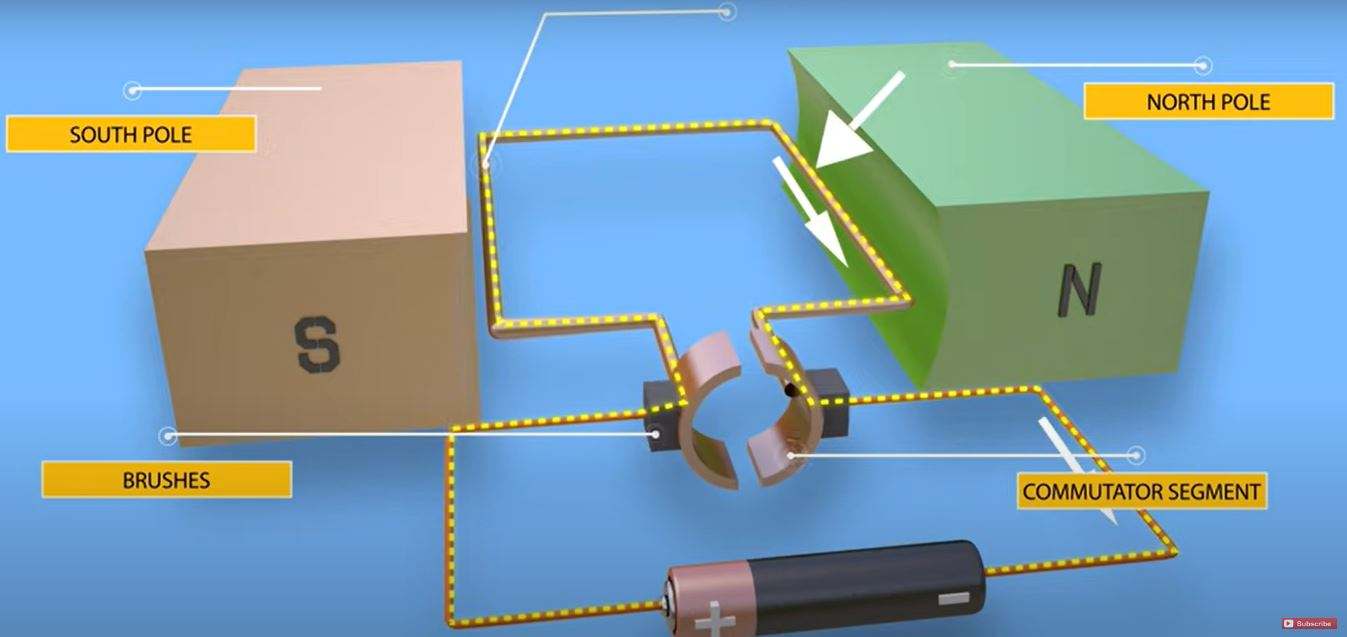
\includegraphics[width=\textwidth]{DCmotor1}
%		\caption{Voltage input}
		%		\label{fig:y equals x}
	\end{subfigure}
	\begin{subfigure}[b]{0.48\textwidth}
		\centering
		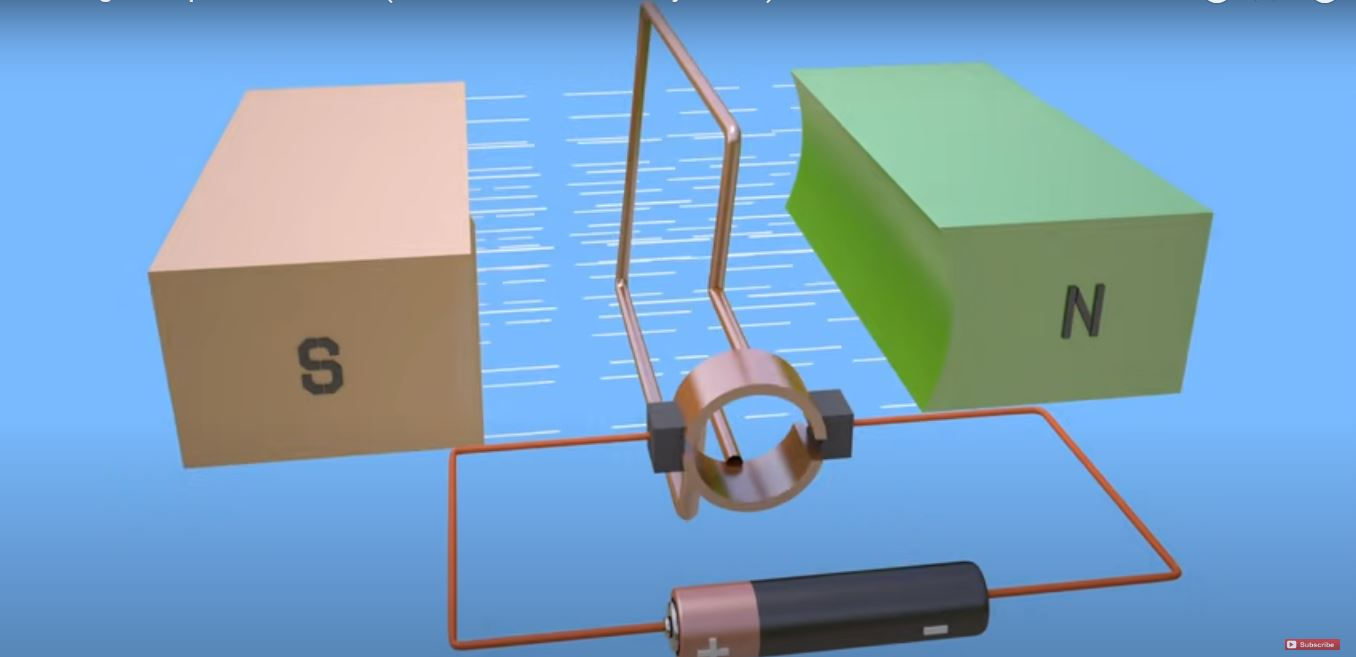
\includegraphics[width=\textwidth]{DCmotor2}
%		\caption{Short circuit}
		%		\label{fig:three sin x}
	\end{subfigure}
		\caption{DC motor scheme. Images from \url{https://youtu.be/j\_F4limaHYI}}
	%	\label{fig:three graphs}
\end{figure}



\end{flushleft}
\end{frame}




\begin{frame}{DC motor mechanical model, 1}
	%\framesubtitle{How do we know the state?}
	\begin{flushleft}
		
		We can describe the dynamics of the motor shaft:
		
		\begin{equation}
			J \frac{d}{dt} \omega = \tau
		\end{equation}
	%
	where $J$ is moment of inertia, $\omega$ is angular velocity and $\tau$ is torque. If we additionally consider linear viscous friction $F \omega$, we get:
	
	\begin{equation}
		J \frac{d}{dt} \omega + F \omega = \tau
	\end{equation}

	The torque $\tau$ can be modeled as a linear function of current in the motor winding:
	 
	 \begin{equation}
	 	\tau = C_\tau I
	 \end{equation}
	 %
	 where $C_\tau$ is torque coefficient.
		
	\end{flushleft}
\end{frame}



\begin{frame}{DC motor mechanical model, 2}
	%\framesubtitle{How do we know the state?}
	\begin{flushleft}
		
		Note that as long as the variable is angular velocity of the shaft $ \omega$, the dynamics is a first-order ODE. If we instead consider orientation of the shaft $\varphi$, the result is a second-order ODE.
		
		\begin{align}
			J \frac{d^2}{dt^2} \varphi + F \frac{d}{dt} \varphi &= \tau \\
			\frac{d}{dt} \varphi &= \omega
		\end{align}
		
	\end{flushleft}
\end{frame}



\begin{frame}{DC motor mechanical model, 3}
	%\framesubtitle{How do we know the state?}
	\begin{flushleft}
		
		The ODE $J \frac{d}{dt} \omega + F \omega = \tau$ is equivalent to the model of RL circuit. This means that the frequency response (considering torque as input and angular velocity as output) is:
		
		\begin{equation}
			|W(\alpha)| =
			\frac{1}{\sqrt{J^2\alpha^2 + F^2}}
		\end{equation}
	%
	where $\alpha$ is the input frequency.
	
	\begin{itemize}
		\item As the input frequency goes to infinity, the amplitude gain goes to zero. 
		\item As the input frequency goes to zero, the amplitude gain goes to $\frac{1}{F}$.
	\end{itemize}
	
		
	\end{flushleft}
\end{frame}




\begin{frame}{DC motor electrical model}
	%\framesubtitle{How do we know the state?}
	\begin{flushleft}
		
		DC motor winding is essentially a RL circuit. We can describe the electrodynamics of the motor winding as:
		
		\begin{equation}
			L \frac{d}{dt} I + RI + C_w \omega = u
		\end{equation}
		%
		where $I$ is current in motor winding, $L$ is induction coefficient of the motor winding, $R$ is resistance of the motor winding, $C_w$ is back-EMF coefficient and $u$ is input voltage.
		
		\bigskip
		
		Note that this model also behaves like a RL circuit.
		
	\end{flushleft}
\end{frame}



\begin{frame}{DC motor electro-mechanical model}
	%\framesubtitle{How do we know the state?}
	\begin{flushleft}
		
		Full electro-mechanical model of a DC motor is given by the next system of ODEs:
		
		\begin{equation}
			\begin{cases}
				L \dot I + RI + C_w \omega = u \\
				J \dot \omega + F \omega = C_\tau I
			\end{cases}
		\end{equation}
		
		Laplace transform of this model is:
		
		\begin{equation}
			\begin{cases}
				Ls I(s) + RI(s) + C_w \omega(s) = u(s) \\
				Js \omega(s) + F \omega(s) = C_\tau I(s)
			\end{cases}
		\end{equation}
		
		
	\end{flushleft}
\end{frame}



\begin{frame}{DC motor, transfer functions, 1}
	%\framesubtitle{How do we know the state?}
	\begin{flushleft}
		
		We can describe transfer functions:
		%
		\begin{equation}
			\begin{bmatrix}
				Ls+R & C_w \\
				-C_\tau & Js+F
			\end{bmatrix}
			\begin{bmatrix}
				I(s) \\ \omega(s)
			\end{bmatrix}
		=
			\begin{bmatrix}
				u(s) \\ 0
			\end{bmatrix}
		\end{equation}
		%
		\begin{align}
				\text{det} = (Ls+R)(Js+F)+ C_w C_\tau \\
				\text{inv} = \frac{1}{\text{det}}
				\begin{bmatrix}
					Js+F & -C_w \\
					C_\tau & Ls+R  
				\end{bmatrix} 
%			\\
%			\begin{bmatrix}
%				I(s) \\ \omega(s)
%			\end{bmatrix}
%		=
%		\frac{1}{\text{det}}
%		\begin{bmatrix}
%			(Js+F) u(s) \\
%			C_\tau u(s)  
%		\end{bmatrix}
		\end{align}
	
	Giving us transfer functions:
	
	\begin{align}
		I(s)  = \frac{Js+F}{(Ls+R)(Js+F)+ C_w C_\tau} u(s), \\
		\omega(s)  = \frac{C_\tau}{(Ls+R)(Js+F)+ C_w C_\tau} u(s)
	\end{align}
		
		
	\end{flushleft}
\end{frame}



\begin{frame}{DC motor, transfer functions, 2}
	%\framesubtitle{How do we know the state?}
	\begin{flushleft}
		
		We can open the brackets in the transfer function:
		%
		\begin{align}
			\omega(s)  = \frac{C_\tau}{JL s^2 + (LF+JR)s + FR+C_w C_\tau} u(s)
		\end{align}
	
		\bigskip
		
		With that, we can transform the model back to time domain, giving us a second-order ODE:
		%
		\begin{align}
			JL \ddot \omega  + (LF+JR) \dot \omega  + (FR+C_w C_\tau) \omega =
			C_\tau u 
		\end{align}
		
	\end{flushleft}
\end{frame}



\begin{frame}{DC motor, state-space}
	%\framesubtitle{How do we know the state?}
	\begin{flushleft}
		
		We can write a state-space model with state variables $I$ and $\omega$:
		
		\begin{align}
			\begin{bmatrix}
				\dot I \\ \dot\omega
			\end{bmatrix}
		=
			\begin{bmatrix}
				-R/L & -C_w/L \\
				C_\tau/J & -F/J
			\end{bmatrix}
			\begin{bmatrix}
				I \\ \omega
			\end{bmatrix}
			+
			\begin{bmatrix}
				1/L \\ 0
			\end{bmatrix}
				u
		\end{align}
		
	\end{flushleft}
\end{frame}



\begin{frame}{Angle control}
	%\framesubtitle{How do we know the state?}
	\begin{flushleft}
		
		Orientation of the motor is given by the angle $\varphi$, where $\dot \varphi(t) = \omega(t)$, or equivalently $s \varphi(s) = \omega(s)$. The transfer function from input voltage to angle $\varphi$ is:
		%
		\begin{align}
			\varphi(s)  = \frac{C_\tau}{JL s^3 + (LF+JR)s^2 + (FR+C_w C_\tau)s} u(s)
		\end{align}
		
		The state-space model then becomes:
		%
		\begin{align}
			\begin{bmatrix}
				\dot I \\ \dot\omega \\ \dot \varphi
			\end{bmatrix}
			=
			\begin{bmatrix}
				-R/L & -C_w/L & 0 \\
				C_\tau/J & -F/J & 0 \\
				0 & 1 & 0
			\end{bmatrix}
			\begin{bmatrix}
				I \\ \omega \\ \varphi
			\end{bmatrix}
			+
			\begin{bmatrix}
				1/L \\ 0 \\ 0
			\end{bmatrix}
			u
		\end{align}
		
		
		
	\end{flushleft}
\end{frame}




\begin{frame}{Payload}
	%\framesubtitle{How do we know the state?}
	\begin{flushleft}
		
		Let us consider a payload with moment of inertia $J_p$ and torque $\tau_p$. Then electro-mechanical dynamics of the motor is:
		
		\begin{equation}
			\begin{cases}
				L \dot I + RI + C_w \omega = u \\
				(J+J_p) \dot \omega + F \omega = C_\tau I + \tau_p
			\end{cases}
		\end{equation}
		
		For example, if the payload is a pendulum with mass $m$ and length $l$, the dynamics becomes:
		
		\begin{equation}
			\begin{cases}
				L \dot I + RI + C_w \dot \varphi = u \\
				(J+ml^2) \ddot \varphi + F \dot \varphi = C_\tau I + mgl\sin(\varphi)
			\end{cases}
		\end{equation}
		
		
	\end{flushleft}
\end{frame}




\begin{frame}{Reducer (gearbox)}
	%\framesubtitle{How do we know the state?}
	\begin{flushleft}
		
		A reducer is a mechanism for reducing angular velocity of the output shaft of the motor, while increasing the output torque.
		
		Let us define angular velocity of the output shaft $\omega_o$ and torque of the output shaft $\tau_o$. An ideal reducer is defined as:
		
		\begin{align}
			\omega_o = \frac{1}{N} \omega \\
			\tau_o = N \tau
		\end{align}
	%
	where $N > 1$ is the reduction ratio.
	
	\bigskip
	
	The key idea is that an ideal reducer allows us to model orientation and velocity of the input shaft and the output shaft using the same coordinates.
		
		
	\end{flushleft}
\end{frame}




\begin{frame}{Moment of inertia with a reducer}
	%\framesubtitle{How do we know the state?}
	\begin{flushleft}
		
		Consider a payload with inertial $J_p$ attached to the output shaft of the reducer, rotating at the angular velocity $\omega_o$. The kinetic energy of the entire system is given by:
		
		\begin{align}
			T &= \frac{1}{2} J \omega^2 + \frac{1}{2} J_p \omega_o^2 = \\
			   &=\frac{1}{2} J \omega^2 + \frac{1}{2} \frac{1}{N^2} J_p \omega^2 = \\
			   &= \frac{1}{2} (J + J_p / N^2 )\omega^2
		\end{align}
	
		 Thus, dynamic of the drive becomes:
		 
		\begin{equation}
		\begin{cases}
			L \dot I + RI + C_w \omega = u \\
			(J + J_p / N^2) \dot \omega + F \omega = C_\tau I +  \tau_p / N
		\end{cases}
		\end{equation}		  
		
		
	\end{flushleft}
\end{frame}


\begin{frame}{Read more}
	% \framesubtitle{Local coordinates}
	\begin{flushleft}
		
		\begin{itemize}
			\item \bref{https://ctms.engin.umich.edu/CTMS/index.php?example=MotorSpeed\&section=SystemModeling}{University of Michigan. DC Motor Speed: System Modeling}
			
			\item \bref{https://web.mit.edu/drela/Public/web/qprop/motor1\_theory.pdf}{First-Order DC Electric Motor Model, Mark Drela, MIT Aero \& Astro}
			
			\item \bref{http://www.ece.ualberta.ca/~tchen/ctm/examples/motor/motor.html}{University of Alberta. DC Motor Speed Modeling}
			
			
			
		\end{itemize}
		
		
	\end{flushleft}
\end{frame}


\myqrframe

\end{document}
